\documentclass[prl,aps,twocolumn,floatfix,amsmath,amssymb,superscriptaddress,tightenlines]{revtex4}
\usepackage{graphicx}
\usepackage{epstopdf}
\usepackage{amsfonts}
\usepackage{bm}
\usepackage{color}
\usepackage{ulem}
\begin{document}

\date{\today}
\title{Chord-length scaling in the entanglement entropy of
  two-dimensional gapless systems}

\author{Hyejin Ju}
\affiliation{University of California, Santa Barbara, CA, 93106}

\author{Ann B. Kallin}
\affiliation{Department of Physics and Astronomy, University of Waterloo, Ontario, N2L 3G1, Canada} 

\author{Paul Fendley}
\affiliation{Physics Department, University of Virginia,
  Charlottesville, VA 22904}
\affiliation{Microsoft Research, Station Q, CNSI Building, University of California, Santa Barbara, CA, 93106}

\author{Matthew B. Hastings}
\affiliation{Microsoft Research, Station Q, CNSI Building, University of California, Santa Barbara, CA, 93106}

\author{Roger G. Melko}
\affiliation{Department of Physics and Astronomy, University of Waterloo, Ontario, N2L 3G1, Canada} 

\begin{abstract} 
We show that the entanglement entropy of several two-dimensional
gapless systems contains a logarithmic term that depends 
on the relative size of the entangled region.
Precisely, we show that the Renyi entropy between two
regions of length $x$ and $L-x$ extending around a torus of length
$L$ depends on $\ln(\sin(\pi x/L))$. This logarithmic term is thus
akin to that appearing in one-dimensional systems with conformal symmetry. We
illustrate this with numerical results on the Heisenberg model with
N\'eel order, a free Dirac fermion, and the nearest-neighbor resonating-valence
bond wave function.


 
\end{abstract}
\maketitle

{\it Introduction.} It is now well established that the low-energy
physics of many one-dimensional (1D) quantum many-body systems can be
described by relativistic 1+1 dimensional field theories.  This
correspondence is common at quantum critical points, where in addition
to scale invariance, quantum systems may enjoy {\it conformal}
invariance. Here conformal field theory (CFT) provides an important
universal number, the {\it central charge} $c$, that appears in an astonishing array of physical
quantities \cite{Cardyubiquitous}. A given CFT, and
thus any quantum critical points it describes, can be
characterized by this number. Moreover, a profound result, Zamolodchikov's
$c$-theorem, indicates that $c$ cannot increase in
renormalization-group flows \cite{Zamo}. The central charge thus
provides a valuable tool in identifying which if any conformal field
theory describes a given Hamiltonian. Namely, since it appears in
various physical quantities, it can be measured numerically, and then
compared with the central charges of the (many) known
CFTs. 

Traditionally, numerically extracting $c$ for a 1d quantum
Hamiltonian was done by analyzing the finite-size spectrum
\cite{BCN,Affleck}.  This is often difficult: not only is it a
subleading contribution to the ground-state energy, but requires also
determining the Fermi velocity.
More recently, a more direct method very amenable to numerical
simulation has been utilized.  The central charge can be extracted
directly from the ground-state wavefunction by measuring its Renyi
entanglement entropy, $ S_n = 1/(1-n) \ln \big[ {\rm Tr} \rho_A^n
\big], $ where region $A$ is entangled with its complement, region
$B$.  In particular, the scaling of the Renyi entropy at a 1D critical system,
with total length $L$ and length of region $A$ being $x$, obeys \cite{Korepin,Cardy}
\begin{equation}
S_n = \frac{c}{6}\left({ \frac{1}{1+n} }\right) \ln\Big[ \frac{L}{\pi} \sin\big( \frac{\pi x}{L} \big) \Big]. \label{1Dcft}
\end{equation}
Thus here $c$ appears as the coefficient of the leading
term.  
Numerical measurement of entanglement entropy have become commonplace and 
very accurate in simulations using the density matrix renormalization group (DMRG).
Eq.~\ref{1Dcft} has therefore become the gold standard for identifying
$c$ -- allowing access to the most important universal signature of
the underlying CFT in one simple measurement.



In higher dimensions, the relationship between entanglement entropy
and universal quantities is less concrete.  Although conformal
invariance exists at scale-invariant critical points in the presence
of translational and rotational symmetry, the breaking of these
symmetries in physical systems can make the critical points
non-conformal.  Moreover, even if conformal, precisely which quantity
in general to identify as a central charge is an open question.
Nonetheless, one can still hope that a logarithmic scaling of
entanglement entropy can be used to define an ``effective'' central
charge for non-conformally invariant systems that may contain
universal physics (or perhaps even the equivalent of the $c$-theorem
in higher-dimensions \cite{ryu,Myers}).  Arguments exist that
logarithms similar to Eq.~(\ref{1Dcft}) should emerge due to some
asymptotic restoration of conformal invariance in higher-dimensional
gapless models \cite{Shredder} (although counter examples are known).  However, as
Calabrese and Cardy caution, basic scaling relationships of
higher-dimensional systems need to be carefully checked before
arguments about asymptotic restoration of conformal invariance are
advanced \cite{EE_CFT}.

 \begin{figure}[ht]
   \begin{center}
   \scalebox{1}{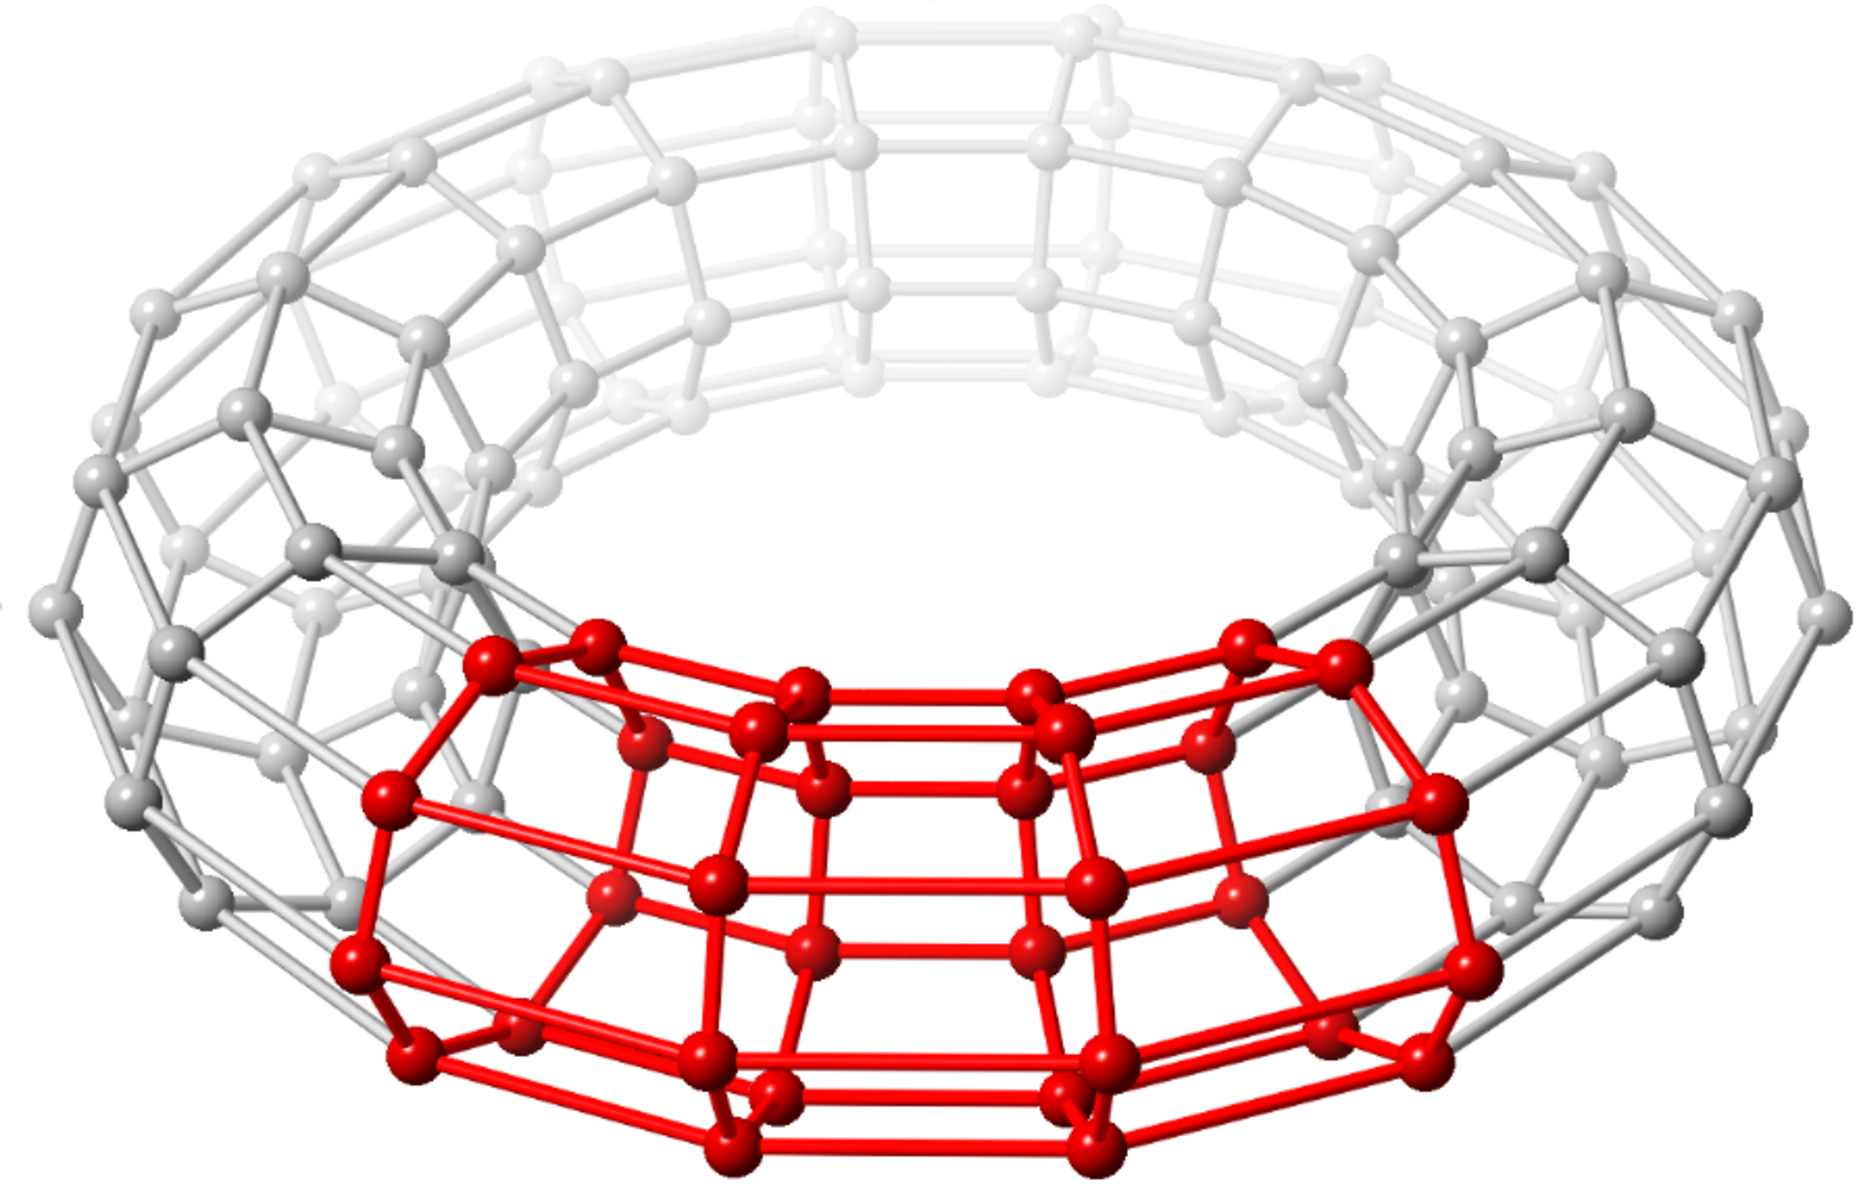
\includegraphics[width=2.3in]{./figs/16x8b.pdf}}
   \end{center}
   \caption{An $8 \times 16$ toroidal simulation cell.  The width of region $A$ (red) is $x=4$.  The boundary length between region $A$ and its complement is $\ell = 16$.  In results in this paper, tori are always square with dimension $L \times L$. }
   \label{fig:torus}
 \end{figure}
 
Since the terms in the Renyi entropy with
universal behavior are subleading in $d>1$, it has only recently become
possible to measure them accurately through the development of measurement
techniques in scalable quantum Monte
Carlo (QMC) methods \cite{swap,XXZ}.  Simulations employing this advance
have confirmed the presence of universal subleading corrections to the
area-law in topologically-ordered systems \cite{isakov}, as well as preliminary
confirmations of area-law (and subleading logarithms) in the simple
gapless 2D N\'eel state \cite{HeisLog}. %>>> Misguich should be mentioned too, they've been doing this for a while???.  
In this paper, we perform a careful
finite-size scaling analysis of Renyi entropies in a specific
cornerless geometry in several gapless wavefunctions \cite{Misguich}.  We show, in
addition to the additive logarithms identified in Ref.~\cite{HeisLog},
the emergence of a ``chord length'' scaling term, which depends on the
width of the region $A$, reminiscent of Eq.~(\ref{1Dcft}) for a 1D
CFT.

Using quantum Monte Carlo (QMC) techniques we simulate both the
Heisenberg ground state and the resonating valence bond (RVB)
wavefunction in two dimensions (2D).  The Heisenberg ground state is
projected from a trial state by applying a high power of the
Hamiltonian, via QMC in the valence bond (VB)
basis \cite{Sandvik}. The VB operators act to reorganize the
bonds while effectively penalizing states with longer bonds.  The RVB
wavefunction contains all possible combinations of only
nearest-neighbor VBs in an equal superpositions \cite{RVB1,RVB2}.  The RVB 
Monte Carlo sampling
algorithm does a random walk through the possible states by creating a
defect at some point and propagating it through the system (thereby
rearranging the nearest-neighbor bonds) until the defect reaches the
initial point and its path forms a closed loop.
If we visualize the Heisenberg ground state in this VB language, then the RVB wavefunction is its largest component, the remainder of the state being equal superpositions with longer bonds decaying as $1/r^3$ \cite{Sandvik} with the length of the bonds.

For both these systems (Heisenberg and RVB) we use a square lattice torus geometry and measure the entanglement % for two different types of region $A$: a $square$ region $A$ containing four corners, and 
using a cornerless $strip$ region $A$ (Fig.~\ref{fig:torus}) which has no corners and constant boundary length $\ell = 2L$ for a given $L$ by $L$ torus.
We denote the width of region $A$ by $x$.
%, where a square will have dimensions $x$ by $x$ and a strip will be $x$ by $L$ when it is embedded in an $L$ by $L$ system.

In Fig.~{\ref{fig:heis_bow}} we illustrate QMC results for the N\'eel state, first explored in Ref.~\cite{HeisLog}.  In that work, the presence of an area law term $\propto \ell$ was confirmed, as well as a subleading logarithmic term $\propto \ln(\ell)$ (present, surprisingly, even with an absence of corners in the region $A$).  This subleading term was extracted when the width of the region $A$, $x = L/2$, is equivalent to the ``center'' of each curve in Fig.~{\ref{fig:heis_bow}}.  As is apparent, this choice of region $A$ removes the $x$-dependence of each curve.  This can be remedied
by the scaling ansatz
\begin{align}
S_2(L) &= a(L) \ell + b(L) \ln(\ell) \nonumber \\
&+ c(L) \ln \left[{ \sin\left({ \frac{\pi x}{L} }\right) }\right] + d(L) \label{Fit}
\end{align}
{\color{red} which we use to fit {\it all} data individually for each system size $L$. }
% 1.  Do we fit all the data individually with this full function?
% 2.  If so that put "each data set individually" if not then "all data simultaneously"
It is clear in Fig.~{\ref{fig:1}} that this form gives an excellent fit to the data for all $x$ and $L$, providing strong evidence for the presence of the chord length.  We can analyze the fits further by examining the dependence of the coefficients on system size $L$.  Most interestingly, we observe the coefficient of the chord-length increasing with $L$, as illustrated in the inset of Fig.~{\ref{fig:1}}.

We next examine the scaling of the Renyi entropy in the RVB wavefunction, illustrated in Fig.~{\ref{fig:2}}.  As apparent in the inset for $L=24$, there exists a more complicated structure to the entropies than in the N\'eel state: the appearance of two branches, an ``upper branch'' when $x$ is odd, and a ``lower branch'' when $x$ is even.  The precise source of the two branches is not known, although simple counting arguments of prototypical valence-bond configurations in the (0,0) topological sector may hint at their existence since the number of valence-bonds crossing from region $A$ to region $B$ alternates strongly with $x$.  Even from this $L=24$ curve there is a clear $x$-dependent curve in each branch: this can be analyzed more closely by examining one branch and attempting fits of the form Eq.~(\ref{Fit}).  In the main plot of Fig.~{\ref{fig:2}}, it is clear that fits to the scaling ansatz for the lower branch are excellent.  Examining the $L$-dependence of the fit coefficients shows that, like in the N\'eel state, the coefficient of the chord length increases with increasing system size.

{\bf Matt}? DIRAC FERMIONS?

% \begin{figure}[ht]
%   \begin{center}
 %  \scalebox{1}{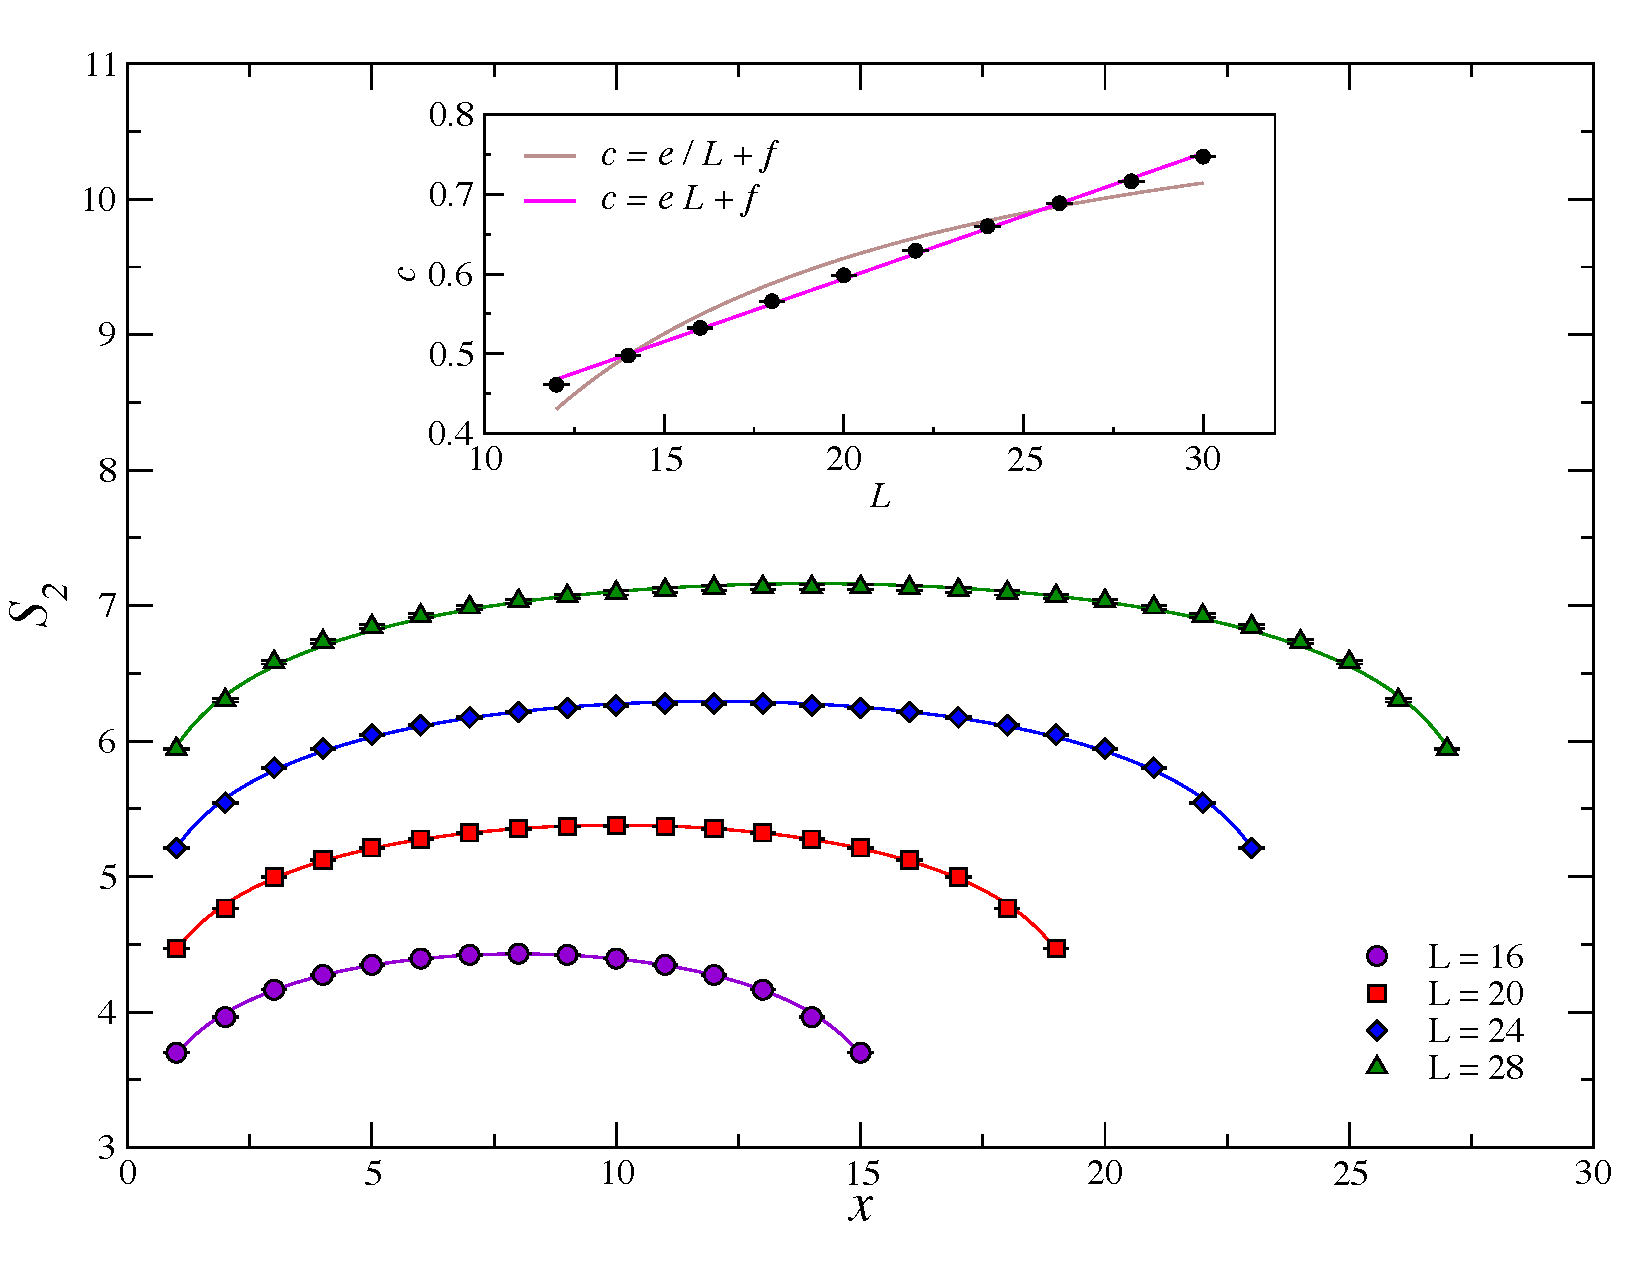
\includegraphics[width=\columnwidth]{./figs/heisenberg.pdf}}
 %  \end{center}
 %  \caption{Heisenberg Renyi-bow. }
 %  \label{fig:1}
% \end{figure}

 \begin{figure}[ht]
   \begin{center}
   \scalebox{1}{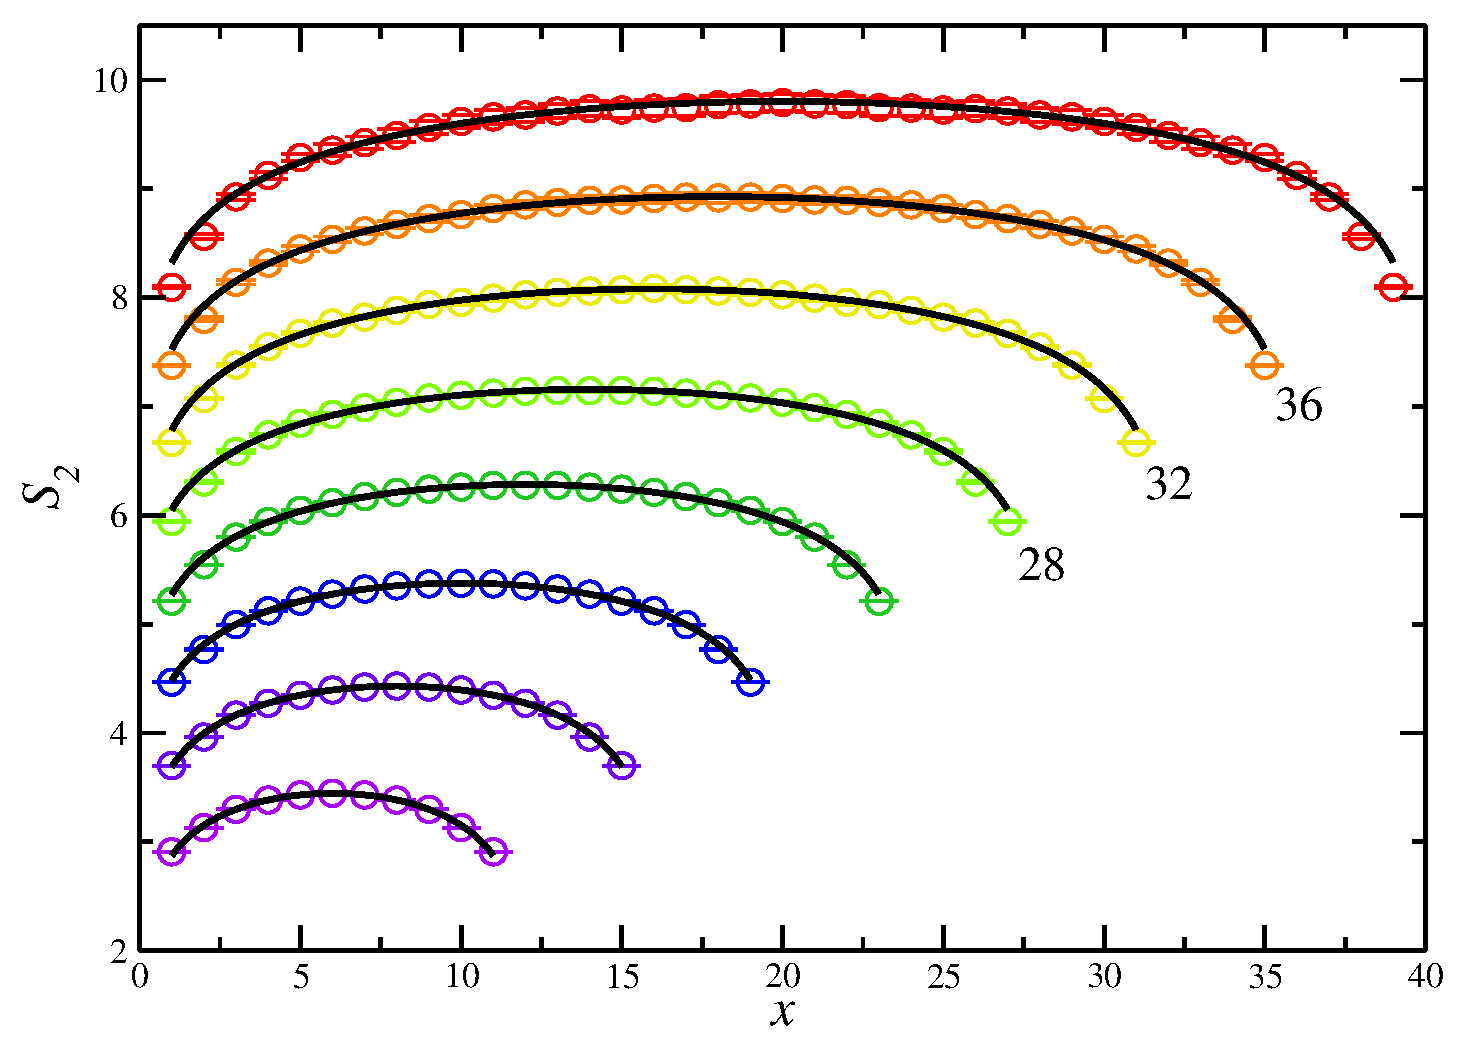
\includegraphics[width=\columnwidth]{./figs/heisenberg/heisbow.eps}}
   \end{center}
   \caption{Heisenberg strip data for $L=12,16,\dots,40$ with fits to the function $m\log(\tfrac{L}{\pi}\sin(\tfrac{x\pi}{L}))+h$} for each system size.
   \label{fig:heis_bow}
 \end{figure}

 \begin{figure}[ht]
   \begin{center}
   \scalebox{1}{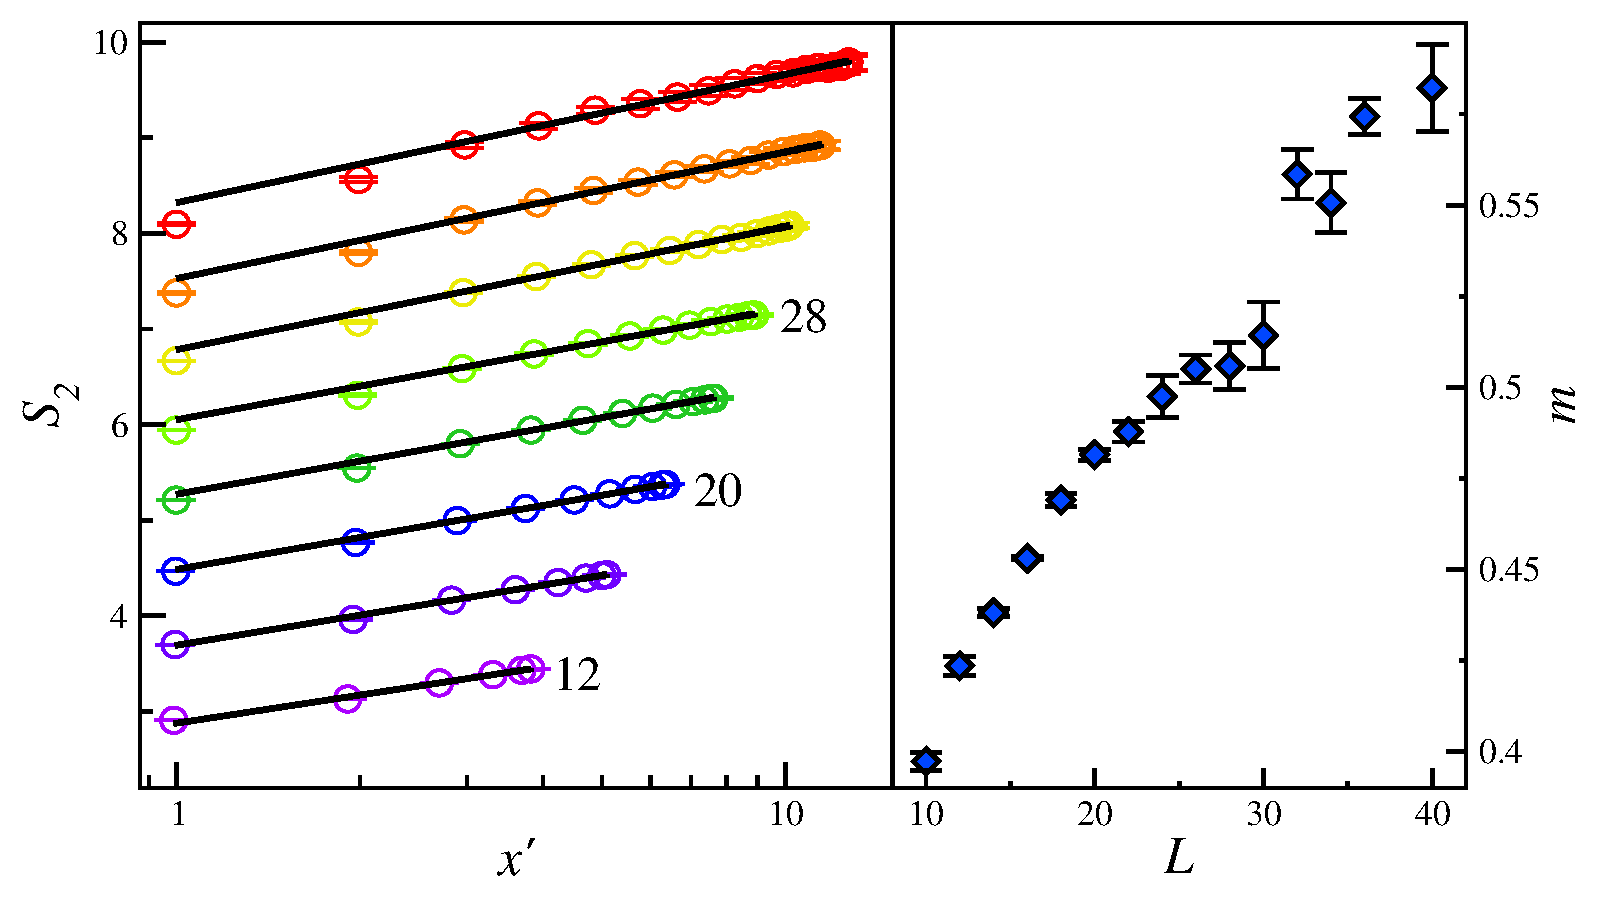
\includegraphics[width=\columnwidth]{./figs/heisenberg/hlines.eps}}
   \end{center}
   \caption{(Left)Heisenberg data and linear fits (excluding the first two data points) for $L=12,16,\dots,40$ plotted in terms of conformal distance, $x^\prime$.
   (Right) Slopes, $m$, for each $L$ on the left {\color{red} and fit to the function $c(L)=L^f+g$}. 
   }
   \label{fig:heis_lines}
 \end{figure}

 \begin{figure}[ht]
   \begin{center}
   \scalebox{1}{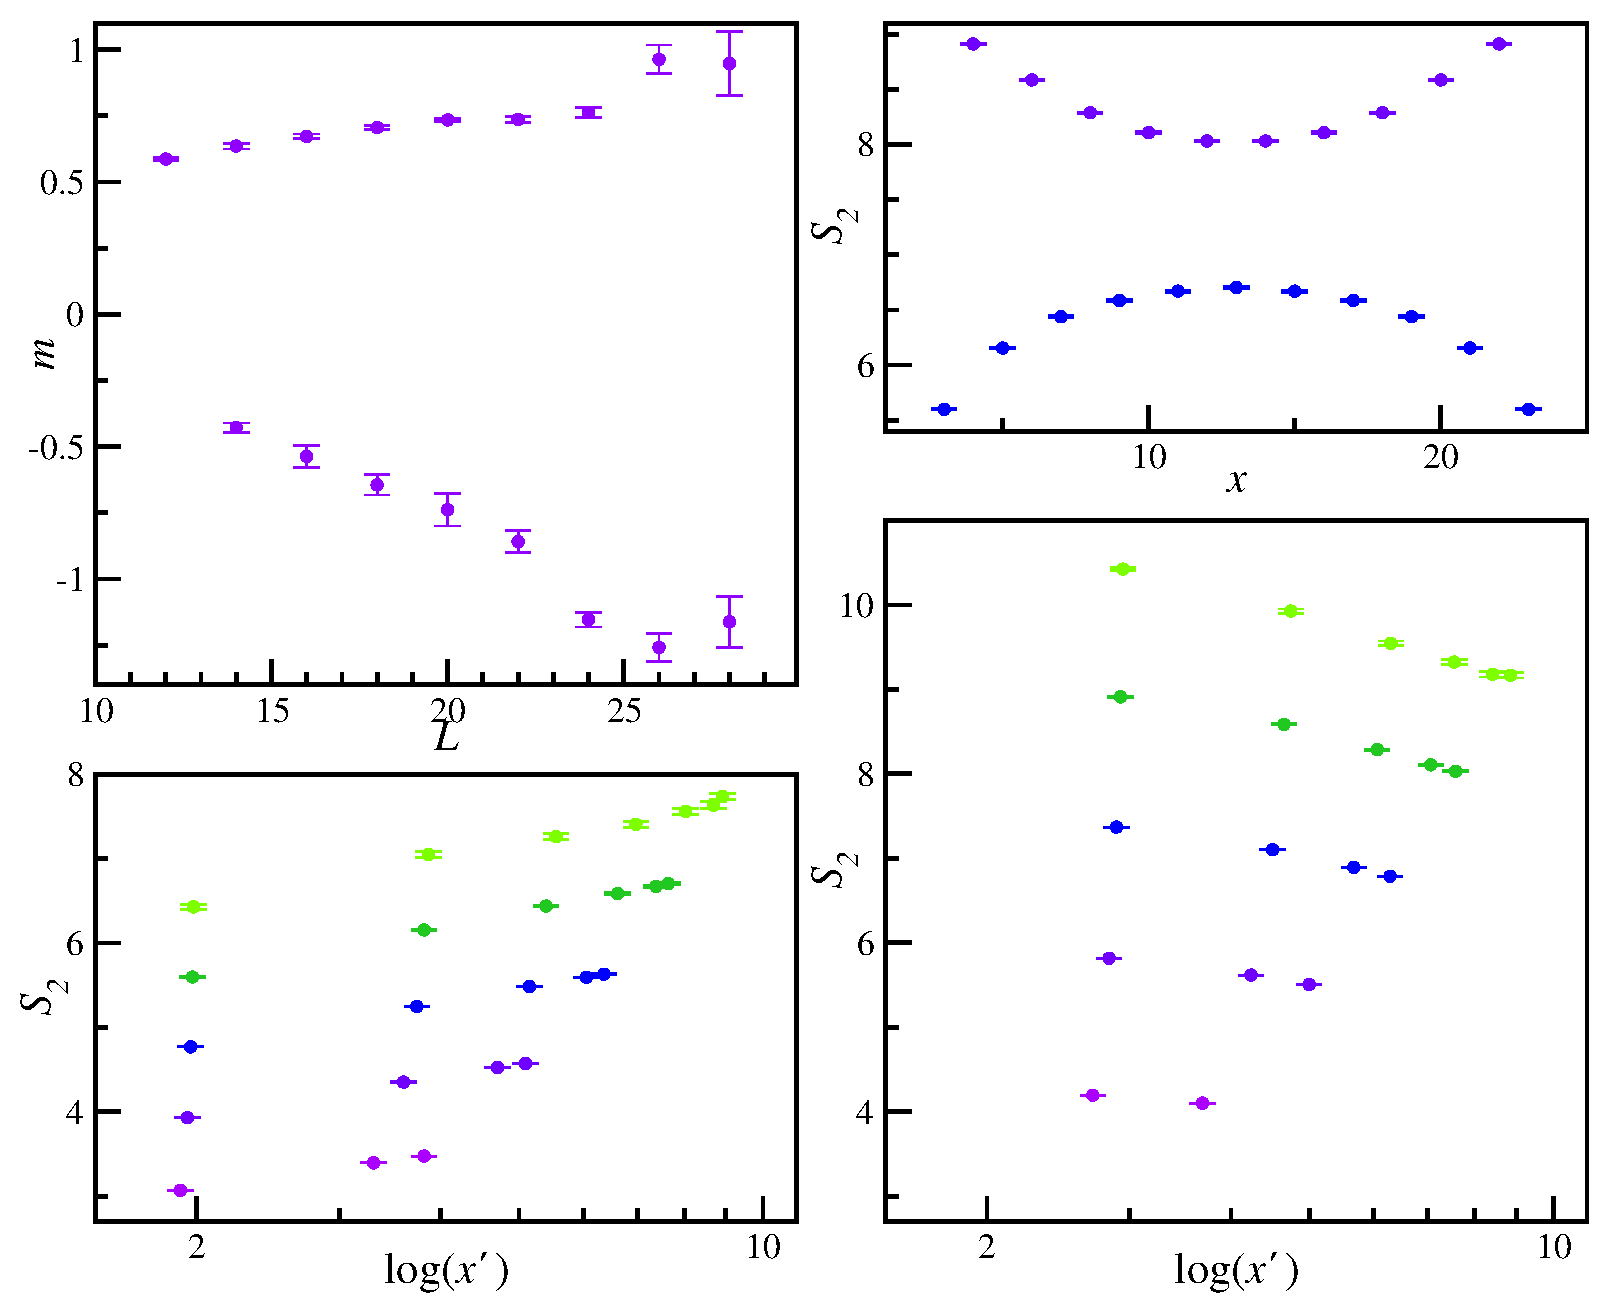
\includegraphics[width=\columnwidth]{./figs/rvb/rvb_fig.eps}}
   \end{center}
   \caption{Preliminary RVB fig - (top left) Slopes from data in bottom panels, (top right) RVB $S_2$ for $L=24$ (excluding $x=1$ and $x=23$). (Bottom) RVB data for $L=12,16,20,24,28$ for even (left) and odd (right) values of $x$.}
   \label{fig:2}
 \end{figure}

{\it Acknowledgments} 
The authors thank R.~Myers and A.~Del Maestro for enlightening discussions. 
R.G.M. would like to acknowledge the support of Microsoft Station Q.
This work has been supported by the Natural Sciences and Engineering
Research Council of Canada (NSERC), and by the US NSF via grants DMR/MPS-0704666 and DMR/MPS1006549.  Simulations were performed on the computing facilities of SHARCNET.


\bibliography{rvb_bib}

\end{document}
